\documentclass[presentation.tex]{subfiles}


\begin{document}
	\begin{frame}[fragile]
		\frametitle{Všeobecná trieda pre $L^1$ a $L^{\infty}$ lineárnu regresiu}
        \begin{python}
from models.models import L1Model, LInfModel
        \end{python}
        \begin{columns}
            \begin{column}{0.55\textwidth}
                \begin{itemize}
                    \item zovšeobecnenie problému
                    \item voľnosť dimenzionality
                    \item vstupný vektor $y$ a matica $\mathbf{X}$
                    \item hodnoty $\beta$ výstupom
                \end{itemize}
            \end{column}

            \begin{column}{0.45\textwidth}
                \begin{python}
# inicializacia
model1 = L1Model(y, X)
model2 = LInfModel(y, X)
# riesenie
beta1 = model1.solve()
beta2 = model2.solve()
                \end{python}
            \end{column}
        \end{columns}
	\end{frame}

    \begin{frame}[fragile]
        \frametitle{Všeobecná trieda pre $L^1$ a $L^{\infty}$ lineárnu regresiu}
        \begin{columns}
        	\begin{column}{0.5\textwidth}
        		\begin{itemize}
        			\item hodnota $R^2$
        			\item vizualizácia pre 2D a 3D
        		\end{itemize}
        	\end{column}
        	\begin{column}{0.5\textwidth}
        		\vspace{0.4cm}
        		\begin{lstlisting}            	
model.r2()
model.visualize()
        		\end{lstlisting}
        	\end{column}
        \end{columns}

        \begin{columns}
            \begin{column}{0.5\textwidth}
            	\centering
                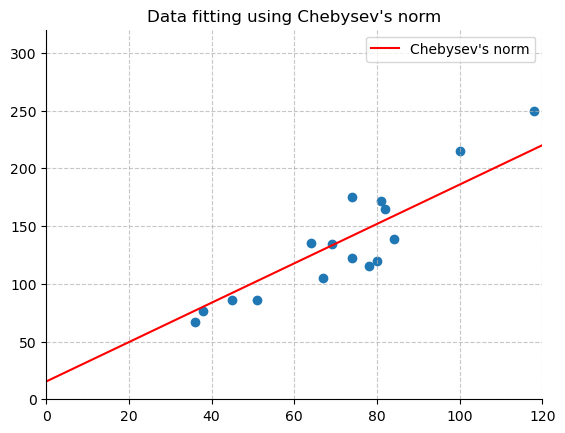
\includegraphics[height=4cm, keepaspectratio]{2D_viz.png}
            \end{column}
            \begin{column}{0.5\textwidth}
            	\centering
                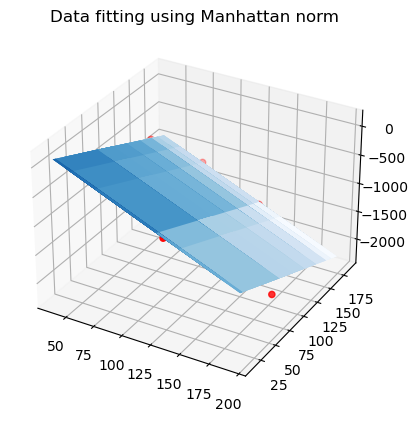
\includegraphics[height=4cm, keepaspectratio]{3D_viz.png}
            \end{column}
        \end{columns}
    \end{frame}
\end{document}